\documentclass[12pt, a4paper, hidelinks]{article}

\usepackage[icelandic]{babel}
\usepackage[T1]{fontenc}
\usepackage[utf8]{inputenc}


\usepackage{amsmath, amssymb, amsfonts}
\usepackage{mathtools}

\usepackage{minted}
\renewcommand{\listingscaption}{Forrit}

\usepackage{url}
\usepackage{hyperref}
\usepackage[hang, flushmargin]{footmisc}
\usepackage[labelfont=sc]{caption}


\usepackage{xcolor}
\usepackage{tabularx}
\usepackage{float}
\usepackage{graphicx}
\usepackage{booktabs}
\usepackage{enumerate}
\usepackage{multirow}
\usepackage{tikz}

\usepackage{times, mathptmx}
\usepackage[scaled=0.85]{beramono}

\usepackage{fancyhdr}
\pagestyle{fancy}
\fancyhf{}
\fancyhead[L]{Kári Hlynsson}
\fancyhead[C]{TÖL203G HEIMADÆMI 4}
\fancyhead[R]{\today}
\fancyfoot[C]{\thepage}

\newcommand{\doctitle}{\uppercase{Heimadæmi 3}}
\newcommand{\coursename}{Tölvunarfræði 2}
\newcommand{\coursenum}{TÖL203G}

% ——— Mengjatákn
\newcommand{\N}{\mathbb{N}}
\newcommand{\Z}{\mathbb{Z}}
\newcommand{\Q}{\mathbb{Q}}
\newcommand{\R}{\mathbb{R}}
\newcommand{\C}{\mathbb{C}}

% ——— Vigrar
\renewcommand{\u}{\mathbf{u}}
\renewcommand{\v}{\mathbf{v}}
\renewcommand{\b}{\mathbf{b}}
\newcommand{\w}{\mathbf{w}}
\newcommand{\p}{\mathbf{p}}
\newcommand{\x}{\mathbf{x}}
\newcommand{\y}{\mathbf{y}}
\newcommand{\z}{\mathbf{z}}

\title{}

\begin{document}
\thispagestyle{plain}
\centerline{\bfseries\Large\doctitle}
\medskip
\centerline{\large\coursenum\ \coursename}
\bigskip

\centerline{\large Kári Hlynsson\footnote{Slóð á Github kóða: \url{https://github.com/lvthnn/TOL203G/tree/master/HD4}}}
\bigskip
\centerline{Háskóli Íslands}
\medskip
\centerline{\today}


\section*{Verkefni 1}

\begin{enumerate}[(a)]
    \item Bætið við klasann \texttt{Card} úr æfingadæminu aðferðinni \texttt{toString()}, sem skilar
    streng með gildi spilsins sem hægt er að prenta út. Þið getið notað ensku upphafsstafina fyrir spaða
    (S), hjarta (H), tígul (D) og lauf (C). Sömuleiðis fyrir mannspilin: ás (A), kóngur (K), drottning (Q)
    og gosi (J). Þannig á aðferðin að skila ,,H-K'' fyrir hjartakóng, ,,C-5'' fyrir laufafimmu o.s.frv.

    \item Skrifið forritið \texttt{CardDeal}, sem tekur á skipanalínunni töluna $k$ sem er á bilinu 1 til 52.
    Forritið prentar þá út $k$ spil sem valin eru af handahófi úr spilastokki. Til þess að við prentum ekki sömu
    spilin út aftur, þá er best að búa til 52-spila fylki. Það er fyllt af öllum mögulegum spilum í venjulegri röð
    og þetta fylki er síðan stokkað. Til þess getið þið notað aðferðina shuffle úr \texttt{StdRandom}. Síðan prentar
    forritið út $k$ fyrstu stökin í fylkinu. Skilið kóðanum fyrir forritið og skjáskoti af keyrslu.
\end{enumerate}

\subsection*{Lausn}
\subsubsection*{Hluti (a)}
Útfærsluna má sjá í \textsc{Forriti} \ref{forrit:Card_toString} fyrir neðan.

\begin{listing}[H]
    \centering
    \inputminted[linenos, breaklines, firstline=21, lastline=25]{java}{../src/V1/Card.java}
    \caption{Útfærsla á \texttt{toString()} í \texttt{Card} klasanum}
    \label{forrit:Card_toString}
\end{listing}

\subsubsection*{Hluti (b)}
Útfærsluna má sjá fyrir neðan í \textsc{Forriti} \ref{forrit:CardDeal}.

\inputminted[linenos]{java}{../src/V1/CardDeal.java}
\captionof{listing}{Útfærsla á \texttt{CardDeal} klasanum\label{forrit:CardDeal}}

\bigskip
\noindent
\textsc{Mynd} \ref{mynd:CardDeal_keyrsla} sýnir síðan keyrslu í skel fyrir neðan.

\begin{figure}[H]
    \centering
    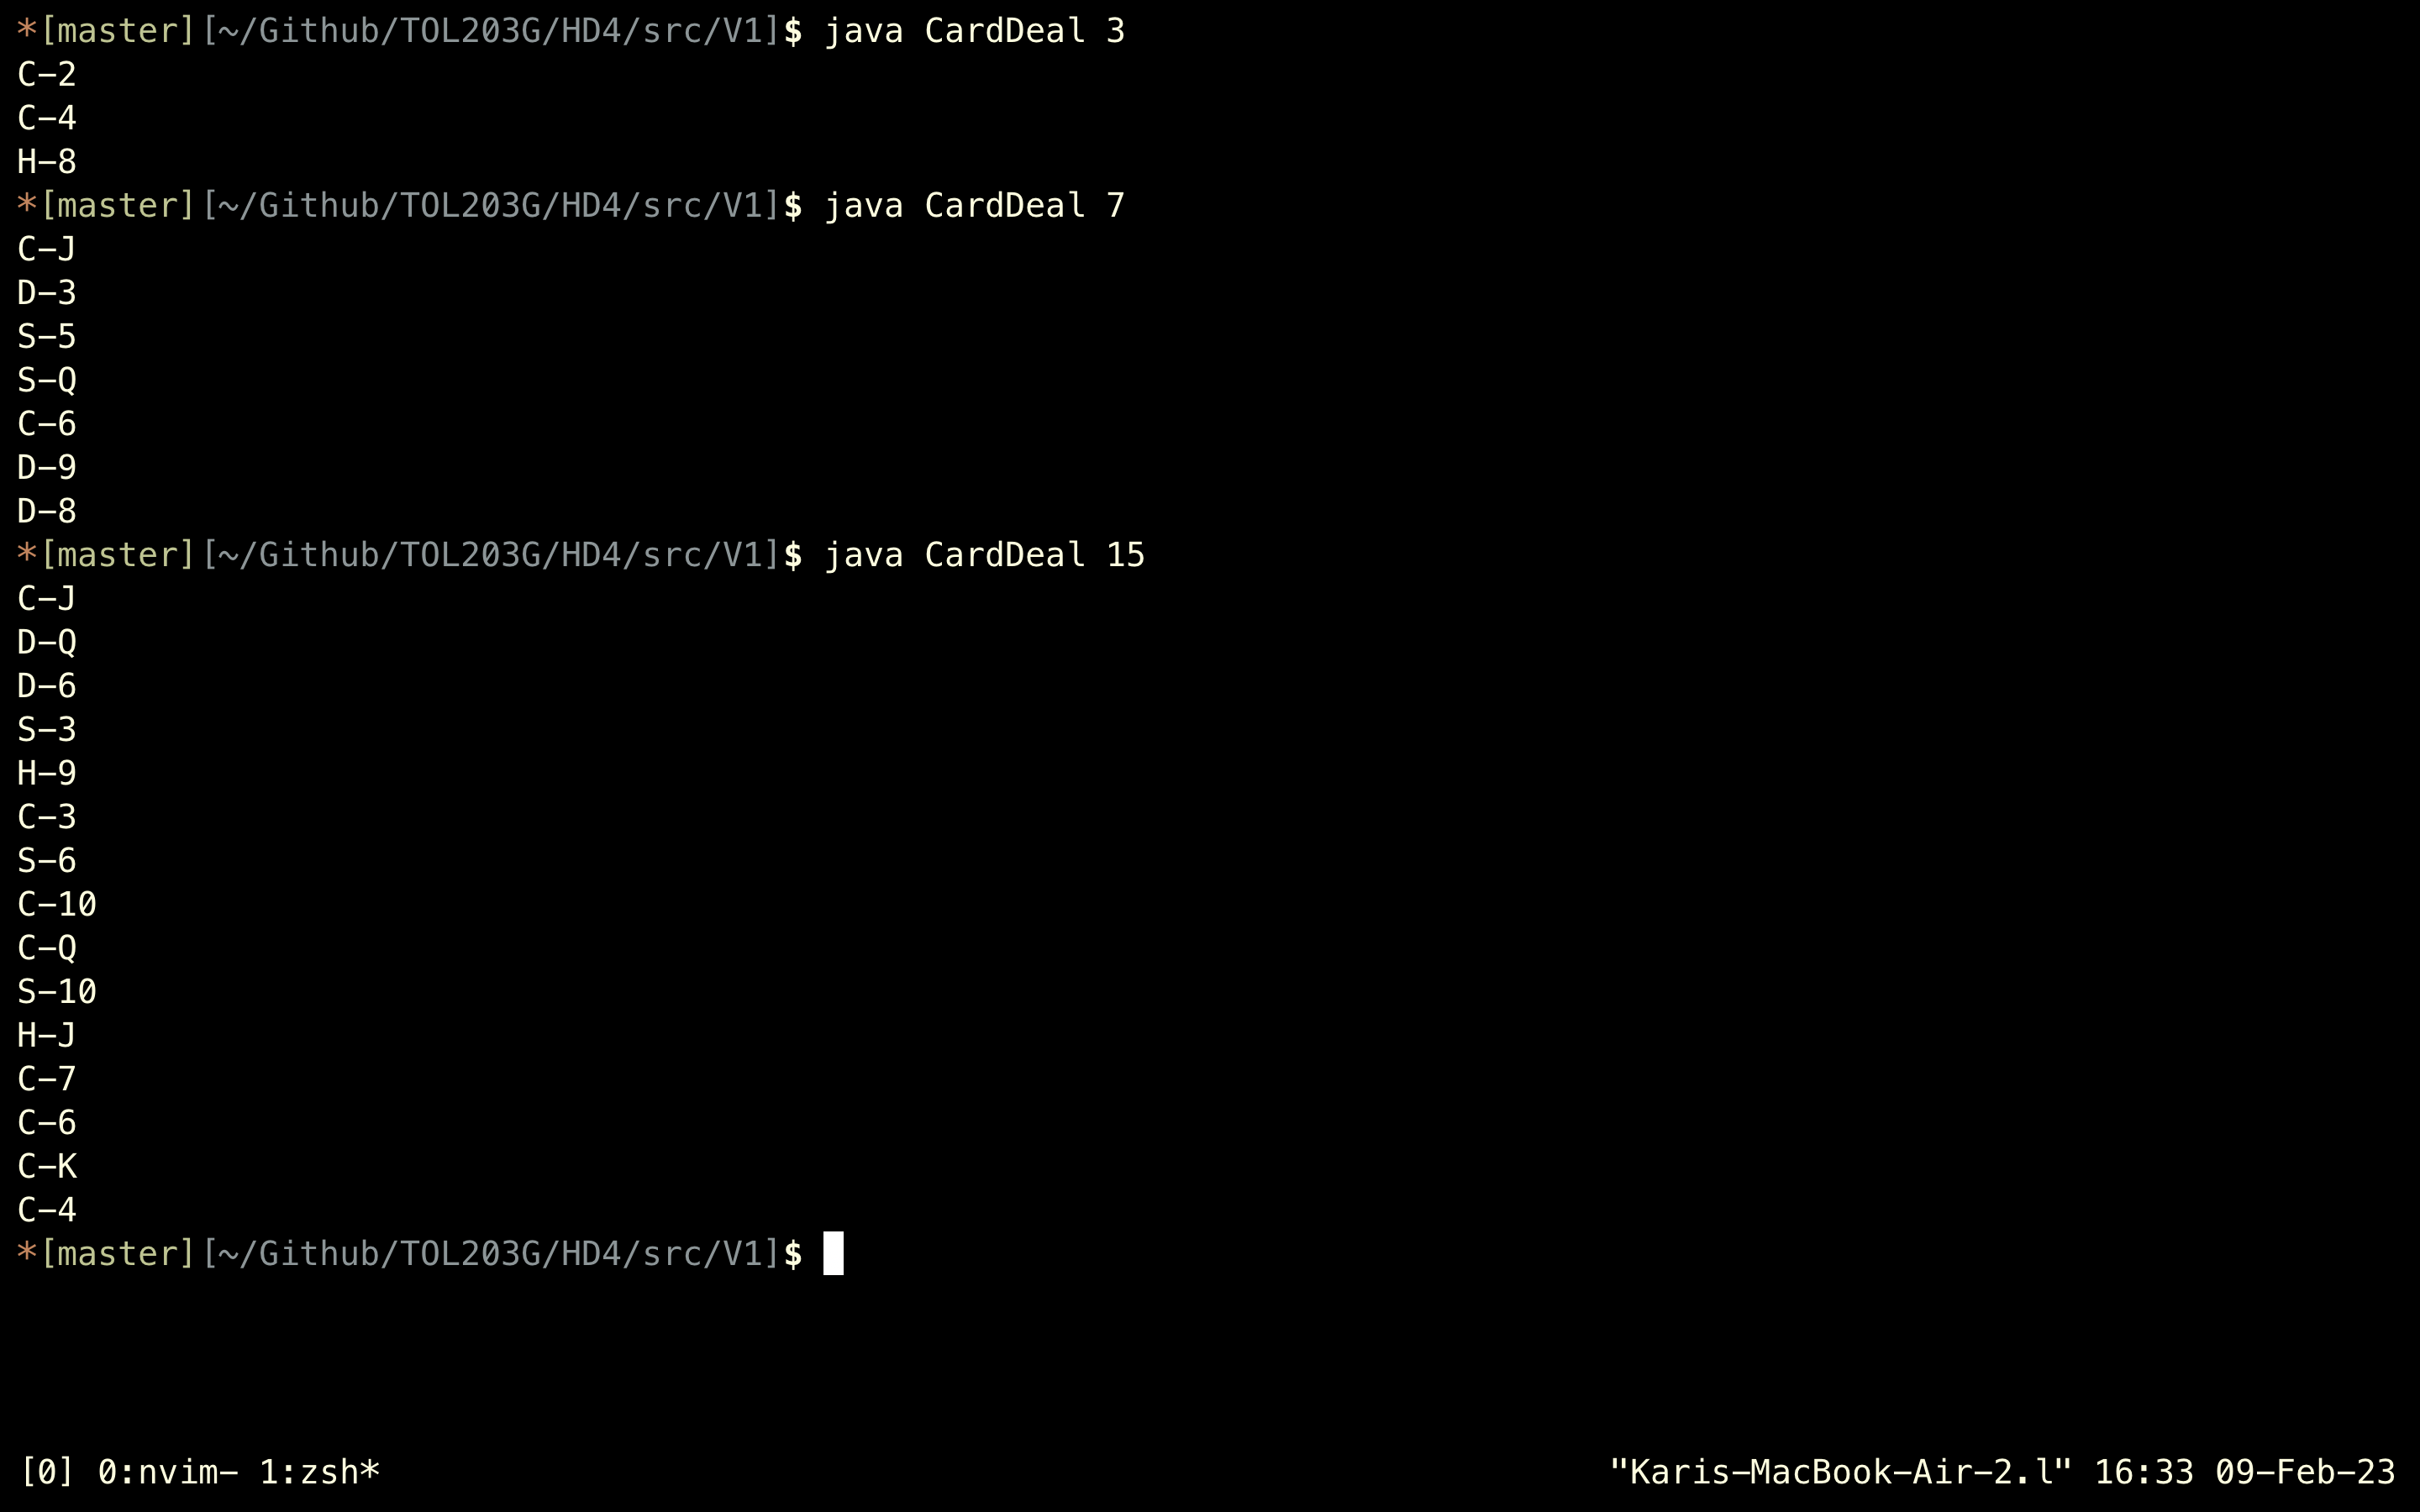
\includegraphics[width=\textwidth]{img/CardDeal_keyrsla.png}
    \caption{Keyrsla á \texttt{CardDeal} í skel fyrir inntök $3, 7, 15$}
    \label{mynd:CardDeal_keyrsla}
\end{figure}

\newpage

\section*{Verkefni 2}
Í útfærslunni á Valröðun í bókinni þá er ekki athugað hvort við þurfum að víxla á stökum \texttt{a[i]} og \texttt{a[min]}.
Ef \texttt{i} er jafnt og \texttt{min} þá er þessi víxlun óþörf. Bætið við \texttt{if}-setningu á undan víxlunarskipuninni
í röðunarfallinu \texttt{sort} sem athugar hvort það þurfi að víxla. Bætið tímamælingarkóða við báðar útgáfurnar og keyrið þær
svo á skránni \texttt{32Kints.txt} og athugið hvort það sé einhver hraðamunur. Þið ættuð að keyra hvora útgáfu a.m.k. þrisvar
sinnum og taka meðaltalið, því það er alltaf einhver breytileiki í keyrslutímanum. Skilið breytta fallinu og niðurstöðum
tímamælinganna.

% meðaltal sort original 2.1794999999999995
% meðaltal sort fast	    0.6352

\newpage

\section*{Verkefni 3}
Þetta er spurning um hegðun valröðunar og innsetningarröðunar á tilteknu $N$-staka inntaksfylki:
\begin{enumerate}[(a)]
    \item Öll stökin í fylkinu hafa sama gildi:
    \begin{enumerate}[(i)]
        \item Hversu marga samanburði notar valröðun?
        \item Hversu marga samanburði notar innsetningarröðun?
    \end{enumerate}
    \item Fylkið er óraðað en inniheldur aðeins tvö ólík gildi, $A$ og $B$. Fjöldi staka af hvoru
    gildi er óþekktur:
    \begin{enumerate}[(i)]
        \item Hversu marga samanburði notar valröðun?
        \item Hversu marga samanburði notar innsetningarröðun?
    \end{enumerate}
\end{enumerate}

\subsection*{Lausn}
\subsubsection*{Hluti (a)}
    \begin{enumerate}[(i)]
        \item Valröðun notar alltaf sama fjölda samanburða því það ítrar frá vísinum \texttt{i}
        og út í enda fylkisins. Fjöldi samanburða er því sem áður $(N - 1) + (N - 2) + \cdots + 2 + 1 \sim N^2/2$.
        \item Innsetningarröðun stöðvar alltaf ef \texttt{a[j]} $\leq$ \texttt{a[j - 1]}, svo í þessu tilviki myndum við alltaf
        bara líta eitt stak aftur fyrir okkur í röðun á fylkinu. Því er heildarfjöldi samanburða $N - 1 \sim N$.
    \end{enumerate}
\subsubsection*{Hluti (b)}
    \begin{enumerate}[(i)]
       \item Eins og áður sagði er valröðun ekki háð inntaki og því höfum við aftur fjölda samanburða $(N - 1) + (N - 2) + \cdots + 2 + 1 \sim N^2/2$.
       \item Látum $n$ og $m$ tákna fjöldann af gildunum $A$ og $B$ í fylkinu, í þeirri röð. Þá er $N = n + m$ heildarföldi staka í fylkinu. Án skerðingar á
       víðgildni athugum við að ef $n \gg m$ þá erum við nokkurn veginn að fást við (ii) í (a)-lið. Ef svo er ekki og $a \approx m$ þá er fjöldi samanburða áður
       en stak finnur sinn stað í raðaða fylkinu $\frac 12 (N - i)$. Við fáum því að heildarfjöldi samanburða er $\frac 12 (N - 1) + \frac 12 (N - 2) + \cdots + 1 + \frac 12 \sim N^2/4$.
    \end{enumerate}

\newpage

\section*{Verkefni 4}
Við getum skilgreint röðunarreikniritið \emph{Slembiröðun}, sem virkar þannig að á meðan fylkið
er ekki raðað þá veljum við tvo vísa \texttt{i} og \texttt{h} af handahófi (á milli $0$ og $N - 1$). Ef
stök \texttt{a[i]} og \texttt{a[j]} eru í langri röð í fylkinu þá víxlum við á þeim og höldum áfram. Forritið
þetta reiknriti í Java (þið getið notað \texttt{Selection.java} sem fyrirmynd). Takið tímann á keyrslu á \texttt{1Kints.txt}.
Keyrið forritið ykkar a.m.k. 5 sinnum og skoðið breytileikann á tímanum. Skilið Java kóðanum fyrir fallið og tímunum á keyrslunum.

\newpage

\section*{Verkefni 5}
Nota á Shell röðun með $3x + 1$ skrefstærðum á 10-staka fylki. Þá eru tvær skrefstærðir: 1 og 4 (reyndar er byrjað með $h = 4$).
\begin{enumerate}[(a)]
    \item Hvert er besta inntak fyrir þessa tegund af Shellröðun? Rökstyðjið og sýnið heildarfjölda
    samanburða fyrir 10-staka fylki.
    \item Sýnið hvernig þessi Shell röðun virkar á 10-staka fylki í öfugri röð (t.d. 10, 9, $\ldots$\@ , 2, 1).
    Sýnið fylkið eftir hvora umferð og fjölda samanburða. Berið fjölda samanburða hér saman við fjölda samanburða
    sem innsetningarröðun myndi nota á þessu fylki.
\end{enumerate}

\subsection*{Lausn}
\subsubsection*{Hluti (a)}
Besta tilvikið kemur upp þegar fylkið er fyrirfram raðað og innri lykkjan keyrir ekki. Kostnaðurinn er einfaldlega að kíkja í gegnum
allar hlutrunurnar svo kostnaðurinn er $\Theta(N)$.

\subsubsection*{Hluti (b)}
Setjum upp rakningar af hlutröðunum í \textsc{Töflu} \ref{tafla:1rodun} og \textsc{Töflu} \ref{tafla:4rodun} hér fyrir neðan.

\newcommand{\threecolumnline}{\multicolumn{3}{c}{\leaders\hbox{\rule[0.4em]{.1pt}{0.4pt}}\hfill\mbox{}}}

\begin{table}[ht!]
    \centering
    \begin{tabular}{l|cccccccccc}
        \toprule
        \multirow{4}{*}{$h = 4$} & 10 & 9 & 8 & 7 & 6 & 5 & 4 & 3 & 2 & 1 \\
              & 10 & \threecolumnline & 6 & \threecolumnline & 2 &  \\
              &    & 9 & \threecolumnline & 5 & \threecolumnline & 1 \\
              \cmidrule{2-11}
              & 2 & 1 & 8 & 7 & 6 & 5 & 4 & 3 & 10 & 9 \\
        \bottomrule
    \end{tabular}
    \caption{Fyrsta $h$-röðunin með $h = 4$.}\label{tafla:4rodun}
\end{table}
\noindent
Í $4$-röðuninni (\textsc{Tafla} \ref{tafla:4rodun} er fjöldi samanburða 6 því við röðum tveimur hlutrunum sem kosta hver um sig 3 samanburði.
Næst kemur $1$-röðunin í \textsc{Töflu} \ref{tafla:1rodun} fyrir neðan sem er venjuleg innsetningarröðun, en í henni eru framkvæmdir
$25$ samanburðir. Til að sjá betri útskýringu, athuga \textsc{Töflu 3}.

\begin{table}[H]
   \centering
   \begin{tabular}{l|cccccccccc}
        \toprule
        \multirow{3}{*}{$h = 1$} & 2 & 1 & 8 & 7 & 6 & 5 & 4 & 3 & 10 & 9 \\
            & 2 & 1 & 8 & 7 & 6 & 5 & 4 & 3 & 10 & 9 \\
            \cmidrule{2-11}
            & 1 & 2 & 3 & 4 & 5 & 6 & 7 & 8 & 9 & 10 \\
        \bottomrule
   \end{tabular}
   \caption{Seinni röðunin með $h = 1$.}\label{tafla:1rodun}
\end{table}

\newpage

\begin{table}[ht!]
    \centering
    \begin{tabular}[pos]{cc|ccccccccccccc}
    \multicolumn{2}{c}{} & \multicolumn{10}{c}{\texttt{a[]}} \\
    \toprule
    $i$ & $j$ & 0 & 1 & 2 & 3 & 4 & 5 & 6 & 7 & 8  & 9 & Samanburðir, $S$ \\
    \midrule
        &     & 2 & 1 & 8 & 7 & 6 & 5 & 4 & 3 & 10 & 9 \\
    1   & 0   & \color{red}  1 & 2 & \color{lightgray} 8 & \color{lightgray} 7 & \color{lightgray} 6 & \color{lightgray} 5 & \color{lightgray} 4 & \color{lightgray} 3 & \color{lightgray} 10 & \color{lightgray} 9 & 1\\
    2   & 2   & \color{lightgray} 1 & \color{lightgray}  2 & \color{red} 8 & \color{lightgray} 7 & \color{lightgray} 6 & \color{lightgray} 5 & \color{lightgray} 4 & \color{lightgray} 3 & \color{lightgray} 10 & \color{lightgray} 9 & 1 \\
    3   & 2   & \color{lightgray} 1 & \color{lightgray}  2 & \color{red} 7 & 8 & \color{lightgray} 6 & \color{lightgray} 5 & \color{lightgray} 4 & \color{lightgray} 3 & \color{lightgray} 10 & \color{lightgray} 9 & 2\\
    4   & 2   & \color{lightgray} 1 & \color{lightgray}  2 & \color{red} 6 & 7 & 8 & \color{lightgray} 5 & \color{lightgray} 4 & \color{lightgray} 3 & \color{lightgray} 10 & \color{lightgray} 9 & 3 \\ 
    5   & 2   & \color{lightgray} 1 & \color{lightgray}  2 & \color{red} 5 & 6 & 7 & 8 & \color{lightgray} 4 & \color{lightgray} 3 & \color{lightgray} 10 & \color{lightgray} 9 & 4 \\
    6   & 2   & \color{lightgray} 1 & \color{lightgray}  2 & \color{red} 4 & 5 & 6 & 7 & 8 & \color{lightgray} 3 & \color{lightgray} 10 & \color{lightgray} 9 & 5 \\ 
    7   & 2   & \color{lightgray} 1 & \color{lightgray}  2 & \color{red} 3 & 4 & 5 & 6 & 7 & 8 & \color{lightgray} 10 & \color{lightgray} 9 & 6 \\
    8   & 8   & \color{lightgray} 1 & \color{lightgray} 2 & \color{lightgray} 3 & \color{lightgray} 4 & \color{lightgray} 5 & \color{lightgray} 6 & \color{lightgray} 7 & \color{lightgray}  8 & \color{red} 10 & \color{lightgray} 9 & 1\\
    9   & 8   & \color{lightgray} 1 & \color{lightgray} 2 & \color{lightgray} 3 & \color{lightgray} 4 & \color{lightgray} 5 & \color{lightgray} 6 & \color{lightgray} 7 & \color{lightgray}  8 & \color{red} 9 & 10 & 2 \\
    \midrule
    \multicolumn{12}{c}{} & $\sum S = 25$ \\
    \bottomrule
    \end{tabular}
    \caption{Rakning af $1$-röðun í Shell röðun með $N = 10$}
\end{table}
\noindent
Prófum nú að bera þetta saman við fjölda samanburða ef við myndum keyra innsetningarröðun á upprunalega fylkið
sem gefið var í dæminu:

\newcommand{\g}{\color{lightgray}}
\newcommand{\curr}{\color{red}}
\begin{table}[ht!]
    \centering
    \begin{tabular}[pos]{cc|ccccccccccccc}
    \multicolumn{2}{c}{} & \multicolumn{10}{c}{\texttt{a[]}} \\
    \toprule
    $i$ & $j$ & 0 & 1 & 2 & 3 & 4 & 5 & 6 & 7 & 8  & 9 & Samanburðir, $S$ \\
    \midrule
        &     & 10 & 9 & 8 & 7 & 6 & 5 & 4 & 3 & 2 & 1 \\
    1   & 0   & \curr 9 & 10 & \g 8 & \g 7 & \g 6 & \g 5 & \g 4 & \g 3 & \g 2 & \g 1 & 1 \\
    2   & 0   & \curr 8 & 9  & 10 & \g 7 & \g 6 & \g 5 & \g 4 & \g 3 & \g 2 & \g 1 & 2 \\ 
    3   & 0   & \curr 7 & 8  & 9  & 10 & \g 6 & \g 5 & \g 4 & \g 3 & \g 2 & \g 1 & 3\\ 
    4   & 0   & \curr 6 & 7  & 8  & 9  & 10 & \g 5 & \g 4 & \g 3 & \g 2 & \g 1 & 4\\
    5   & 0   & \curr 5 & 6  & 7  & 8  & 9  & 10 & \g 4 & \g 3 & \g 2 & \g 1 & 5 \\
    6   & 0   & \curr 4 & 5 & 6 & 7 & 8 & 9 & 10 & \g 3 & \g 2 & \g 1 & 6 \\
    7   & 0   & \curr 3 & 4 & 5 & 6 & 7 & 8 & 9 & 10 & \g 2 & \g 1 & 7 \\
    8   & 0   & \curr 2 & 3 & 4 & 5 & 6 & 7 & 8 & 9 & 10 & \g 1 & 8 \\
    9   & 0   & \curr 1 & 2 & 3 & 4 & 5 & 6 & 7 & 8 & 9 & 10 & 9 \\
    \midrule
    \multicolumn{12}{c}{} & $\sum S = 45$ \\
    \bottomrule
    \end{tabular}
    \caption{Innsetningarröðun á fylki í öfugri röð með $N = 10$.}
\end{table}
\noindent
Eins og má sjá er sparnaðurinn talsverður við að nota Shell röðun, en það munar 20 samanburðum
á röðunarreikniritunum. $\blacksquare$
\end{document}